\subsection{Details in Derivations}
\label{C3-Appendix_Derivations}

%\subsubsection{The Necessary Conditions of the Current-Value Hamiltonian-Lagrangian for the Social Planner's Problem}
%\label{C3-Appendix_Derivations_Social-Planners-Problem_Necessary-Conditions}

\subsubsection{Linearization near the Steady State of the Social Planner's Problem}
\label{C3-Appendix_Derivations_Linearization-near-the-Steady-State-of-the-Social-Planners-Problem}
Using a Taylor series expansion, $\dot{R}_{t}$ can be approximated near the steady state ($R_{ss}$, $\pi_{ss}$):
\begin{equation*}
\begin{split}
    \dot{R}_{t} \ 
    & \approx \ (-R_{ss} Pr_{ss} \ + \ E) \\
    & \hspace{1.0cm} + \ \frac{\partial}{\partial R_{t}} (-R_{t} Pr_{t} \ + \ E) (R_{t} \ - \ R_{ss}) \ + \ \frac{\partial}{\partial \pi_{t}} (-R_{t} Pr_{t} \ + \ E) (\pi_{t} \ - \ \pi_{ss}) \\
    & = \ 0 \ + \ \left( -Pr_{t} \ - \ \frac{\partial Pr_{t}}{\partial R_{t}} R_{t} \right) (R_{t} \ - \ R_{ss}) \ + \ \left( -\frac{\partial Pr_{t}}{\partial \pi_{t}} R_{t} \right) (\pi_{t} \ - \ \pi_{ss}) \\
    & = \ \left( -Pr_{t} \ - \ \frac{\partial Pr_{t}}{\partial R_{t}} R_{t} \right) (R_{t} \ - \ R_{ss}) \ + \ \left( -\frac{\partial Pr_{t}}{\partial \pi_{t}} R_{t} \right) (\pi_{t} \ - \ \pi_{ss}).
\end{split}
\end{equation*}
In the same way, the linear approximation of $\dot{\pi}_{t}$ near the steady state ($R_{ss}$, $\pi_{ss}$) is given by
\begin{equation*}
\begin{split}
    \dot{\pi}_{t} \ 
    & \approx \ \left(r \pi_{ss} \ - \ \sigma \big( \gamma \ - \ \ln(1 - Pr_{ss}) \big) \right) \\
    & \hspace{1.0cm} + \ \frac{\partial}{\partial R_{t}} \left(r \pi_{t} \ - \ \sigma \big( \gamma \ - \ \ln(1 - Pr_{t}) \big) \right) (R_{t} \ - \ R_{ss}) \\
    & \hspace{1.0cm} + \ \frac{\partial}{\partial \pi_{t}} \left(r \pi_{t} \ - \ \sigma \big( \gamma \ - \ \ln(1 - Pr_{t}) \big) \right) (\pi_{t} \ - \ \pi_{ss}) \\
    & = \ 0 \ + \ \left( -\frac{\sigma}{1 - Pr_{t}} \frac{\partial Pr_{t}}{\partial R_{t}} \right) (R_{t} \ - \ R_{ss}) \ + \ \left( r \ - \ \frac{\sigma}{1 - Pr_{t}} \frac{\partial Pr_{t}}{\partial \pi_{t}} \right) (\pi_{t} \ - \ \pi_{ss}) \\
    & = \ \left( -\frac{\sigma}{1 - Pr_{t}} \frac{\partial Pr_{t}}{\partial R_{t}} \right) (R_{t} \ - \ R_{ss}) \ + \ \left( r \ - \ \frac{\sigma}{1 - Pr_{t}} \frac{\partial Pr_{t}}{\partial \pi_{t}} \right) (\pi_{t} \ - \ \pi_{ss}).
\end{split}
\end{equation*}
From those two approximations, the linearized system near the steady state ($R_{ss}$, $\pi_{ss}$) is
\begin{equation*}
\begin{split}
    \begin{pmatrix}
        \dot{R}_{t} \\
        \dot{\pi}_{t}
    \end{pmatrix} \ 
    & = \ 
    \begin{pmatrix}
        -Pr_{t} \ - \ \frac{\partial Pr_{t}}{\partial R_{t}} R_{t} & -\frac{\partial Pr_{t}}{\partial \pi_{t}} R_{t} \\
        -\frac{\sigma}{1 - Pr_{t}} \frac{\partial Pr_{t}}{\partial R_{t}} & r \ - \ \frac{\sigma}{1 - Pr_{t}} \frac{\partial Pr_{t}}{\partial \pi_{t}}
    \end{pmatrix}
    \begin{pmatrix}
        R_{t} \ - \ R_{ss} \\
        \pi_{t} \ - \ \pi_{ss}
    \end{pmatrix} \\
    & = \
    \begin{pmatrix}
        [1] & [2] \\
        [3] & [4]
    \end{pmatrix}
    \begin{pmatrix}
        R_{t} \ - \ R_{ss} \\
        \pi_{t} \ - \ \pi_{ss}
    \end{pmatrix}.
\end{split}
\end{equation*}

Applying the Implicit Function Theorem to necessary condition (\ref{Equation:Social-Planners-Problem_Meaning-of-Costate-Variable}), we can obtain the followings:
\begin{equation*}
\begin{cases}
    \begin{split}
        \frac{\partial Pr_{t}}{\partial R_{t}} \ 
        & = \ - \frac{ \big( \alpha^{2} u''(\alpha R_{t} Pr_{t}) - c''(R_{t} Pr_{t}) \big) Pr_{t}}{ \ \big( \alpha^{2} u''(\alpha R_{t} Pr_{t}) - c''(R_{t} Pr_{t}) \big) R_{t} \ - \ \frac{\sigma}{Pr_{t}(1 - Pr_{t})} \ } \\
        \frac{\partial Pr_{t}}{\partial \pi_{t}} \
        & = \ \frac{1}{ \ \big( \alpha^{2} u''(\alpha R_{t} Pr_{t}) - c''(R_{t} Pr_{t}) \big) R_{t} \ - \ \frac{\sigma}{Pr_{t}(1 - Pr_{t})} \ } 
    \end{split}
\end{cases}
\end{equation*}
Because $\alpha^{2} u''(\alpha R_{t} Pr_{t}) - c''(R_{t} Pr_{t}) < 0$ in our setting, $\partial Pr_{t} / \partial R_{t} < 0$ and $\partial Pr_{t} / \partial \pi_{t} < 0$.

In the coefficient matrix,
\begin{equation*}
\begin{split}
    [1] \ 
    & : \ \ -Pr_{t} \ - \ \frac{\partial Pr_{t}}{\partial R_{t}} R_{t} \ = \frac{\frac{\sigma}{Pr_{t}(1 - Pr_{t})}}{ \ \big( \alpha^{2} u''(\alpha R_{t} Pr_{t}) - c''(R_{t} Pr_{t}) \big) R_{t} \ - \ \frac{\sigma}{Pr_{t}(1 - Pr_{t})} \ } \ < \ 0; \\
    [2] \
    & : \ \ -\frac{\partial Pr_{t}}{\partial \pi_{t}} R_{t} \ > \ 0; \\
    [3] \
    & : \ \ -\frac{\sigma}{1 - Pr_{t}} \frac{\partial Pr_{t}}{\partial R_{t}} \ > \ 0; \ \text{and} \\
    [4] \ 
    & : \ \ r \ - \ \frac{\sigma}{1 - Pr_{t}} \frac{\partial Pr_{t}}{\partial \pi_{t}} \ > \ 0.
\end{split}
\end{equation*}
Therefore, the determinant of the coefficient matrix clearly has a negative value (i.e., $[1] \times [4] - [2] \times [3] < 0$). 

\subsubsection{The Value Function for a Well Site $i$ in state $k$ in Continuous Time}
\label{C3-Appendix_Derivations_Value-Function-in-Continuous-Time}
In our framework, the instantaneous Bellman equation can be approximated as follows:
\begin{equation*}
\begin{split}
    (1 + \tau \rho) V_{ik} (t) \
    & \approxeq \ \tau (f_{ik} \ + \ \lambda_{a} \tilde{f}_{ik}) \\
    & \hspace{0.7cm} + \ \tau \lambda_{a} E\Big[ \underset{a \in \mathcal{A}}{\max} \left\{ V_{i,\ell(i, a, k)} (t + \tau) \ + \ \psi_{iak} \ + \ \tilde{\psi}_{iak} \ + \ \epsilon_{iak} \right\} \Big] \\
    & \hspace{0.7cm} + \ \sum_{\ell \neq k} \tau \lambda_{k\ell} V_{i\ell}(t + \tau) \\
    & \hspace{0.7cm} + \ \left\{ 1 \ - \ \tau \left( \lambda_{a} \ + \ \sum_{\ell \neq k} \lambda_{k\ell} \right) \right\} V_{ik} (t + \tau),
\end{split}
\end{equation*}
where $1 + \tau \rho$ is the discount factor for the time increment $\tau$, $\tau \lambda_{a}$ is the probability that the firm in state $k$ choose an action $a$ in an incremental time period $\tau$, and $\sum_{\ell \neq k} \tau \lambda_{k\ell}$ is the probability of moving from state $k$ to state $\ell$. The curly bracket of the fourth line in the expression, therefore, means the probability that the firm remains at state $k$. 

Rearranging terms, dividing by $\tau$, and letting $\tau \rightarrow 0$ yield a simpler expression:
\begin{equation*}
\begin{split}
    & -\big\{ V_{ik} (t + \tau) \ + \ V_{ik} (t) \big\} \ + \ \tau \rho V_{ik} (t) \ + \ \tau \left( \lambda_{a} \ + \ \sum_{\ell \neq k} \lambda_{k\ell} \right) V_{ik}(t + \tau) \\
    & \hspace{1.0cm} \approxeq \ \tau (f_{ik} \ + \ \lambda_{a} \tilde{f}_{ik}) \ + \ \tau \lambda_{a} E\Big[ \underset{a \in \mathcal{A}}{\max} \left\{ V_{i,\ell(i, a, k)} (t + \tau) \ + \ \psi_{iak} \ + \ \tilde{\psi}_{iak} \ + \ \epsilon_{iak} \right\} \Big] \\
    & \hspace{1.7cm} + \ \sum_{\ell \neq k} \tau \lambda_{k\ell} V_{i\ell}(t + \tau) \\
    & -\frac{1}{\tau} \big\{ V_{ik} (t + \tau) \ + \ V_{ik} (t) \big\} \ + \ \rho V_{ik}(t) \ + \ \left( \lambda_{a} \ + \ \sum_{\ell \neq k} \lambda_{k\ell} \right) V_{ik}(t + \tau) \\
    & \hspace{1.0cm} \approxeq \ (f_{ik} \ + \ \lambda_{a} \tilde{f}_{ik}) \ + \ \lambda_{a} E\Big[ \underset{a \in \mathcal{A}}{\max} \left\{ V_{i,\ell(i, a, k)} (t + \tau) \ + \ \psi_{iak} \ + \ \tilde{\psi}_{iak} \ + \ \epsilon_{iak} \right\} \Big] \\
    & \hspace{1.7cm} + \ \sum_{\ell \neq k} \lambda_{k\ell} V_{i\ell}(t + \tau) \\
    & -\dot{V}_{ik} (t) \ + \ \left( \rho \ + \ \lambda_{a} \ + \ \sum_{\ell \neq k} \lambda_{k\ell} \right) V_{ik}(t) \\
    & \hspace{1.0cm} = \ (f_{ik} \ + \ \lambda_{a} \tilde{f}_{ik}) \ + \ \lambda_{a} E\Big[ \underset{a \in \mathcal{A}}{\max} \left\{ V_{i,\ell(i, a, k)} (t) \ + \ \psi_{iak} \ + \ \tilde{\psi}_{iak} \ + \ \epsilon_{iak} \right\} \Big] \ + \ \sum_{\ell \neq k} \lambda_{k\ell} V_{i\ell}(t)
\end{split}
\end{equation*}

\subsubsection{The Euler Equation for the Firm's Problem}
\label{C3-Appendix_Derivations_Euler-Equation-for-the-Firms-Problem}
Necessary condition (\ref{Equation:Firms-Problem_Necessary-Conditions_Drilling-Probability}) leads to the following when $R_{t}^{g} > 0$ and $Pr_{t}^{g} \in (0, 1)$:
\begin{equation*}
\begin{split}
    \pi_{t}^{g} \
    & = \ \psi_{t}^{g} \ + \ \sigma (\gamma - \ln(Pr_{t}^{g})) \ - \ \sigma (\gamma - \ln(1 - Pr_{t}^{g})).
\end{split}
\end{equation*}
Under the same conditions, necessary condition (\ref{Equation:Firms-Problem_Necessary-Conditions_Costate-Variable}) is
\begin{equation*}
\begin{split}
    \dot{\pi}_{t}^{g} \ 
    & = \ \rho \pi_{t}^{g} \ - \ \big\{ f_{t}^{g} \ + \ \lambda_{a} \sigma \big( \gamma \ - \ \ln(1 - Pr_{t}^{g}) \big) \big\}.
\end{split}
\end{equation*}
Under the assumption that there is no exogenous price change, taking time derivative to the first equation yields
\begin{equation*}
\begin{split}
    \dot{\pi}_{t}^{g} \ 
    % & = \ \dot{\psi}_{t}^{g} \ - \ \sigma \left( \frac{1}{Pr_{t}^{g}} \ + \ \frac{1}{1 - Pr_{t}^{g}} \right) \dot{Pr}_{t}^{g} \\
    & = \ 0.
\end{split}
\end{equation*}
Due to $\dot{\pi}_{t}^{g} = 0$, substituting the first equation into the second one, with soem algebra, allows us having the Euler equation:
\begin{equation*}
\begin{split}
    \frac{ \ f_{ik} \ + \ \lambda_{a} \sigma \big( \gamma \ - \ \ln(1 - Pr_{k}) \big) \ }{\rho} \
    & = \ \left\{ \psi_{i1k} \ + \ \sigma \big( \gamma \ - \ \ln(Pr_{k}) \big) \right\} \ - \ \sigma \big( \gamma \ - \ \ln(1 - Pr_{k}) \big).
\end{split}
\end{equation*}



\clearpage
\subsection{Additional Figure(s) and Table(s)}
\label{C3-Appendix_Additional-Figures-and-Tables}
%\afterpage{
    \begin{figure}[ht!]
        \centering
        \includegraphics[scale = 0.105]{04_Chapter-3/00A_Figures/Figure_Cross-Sectional-Approach_Estimates-from-Robinson-Estimator_Spatial-Distribution-of-Unobservable-Geological-Quality.png}
        \caption{Spatial Distribution of the Estimated Geological Characteristic by Year}
        \caption*{
        	{\small
            \textit{Note}: 
            This figure illustrates the estimated geologic feature for each horizontal well completed between 2013 and 2016 by year. In this figure, each square is a section in the Public Land Survey System, whereas each dot indicates an individual well's geological characteristic. It is apparent that the share of drilling of horizontal wells with (relatively) small estimates decreased significantly starting in 2014, corresponding to the beginning of the oil price crash.
        }}
        \label{Figure:Spatial-Distribution-of-the-Estimated-Geological-Characteristic-by-Year}
    \end{figure}
%}

\begin{landscape}
%\afterpage{
    \begin{figure}[t!]
        \centering
        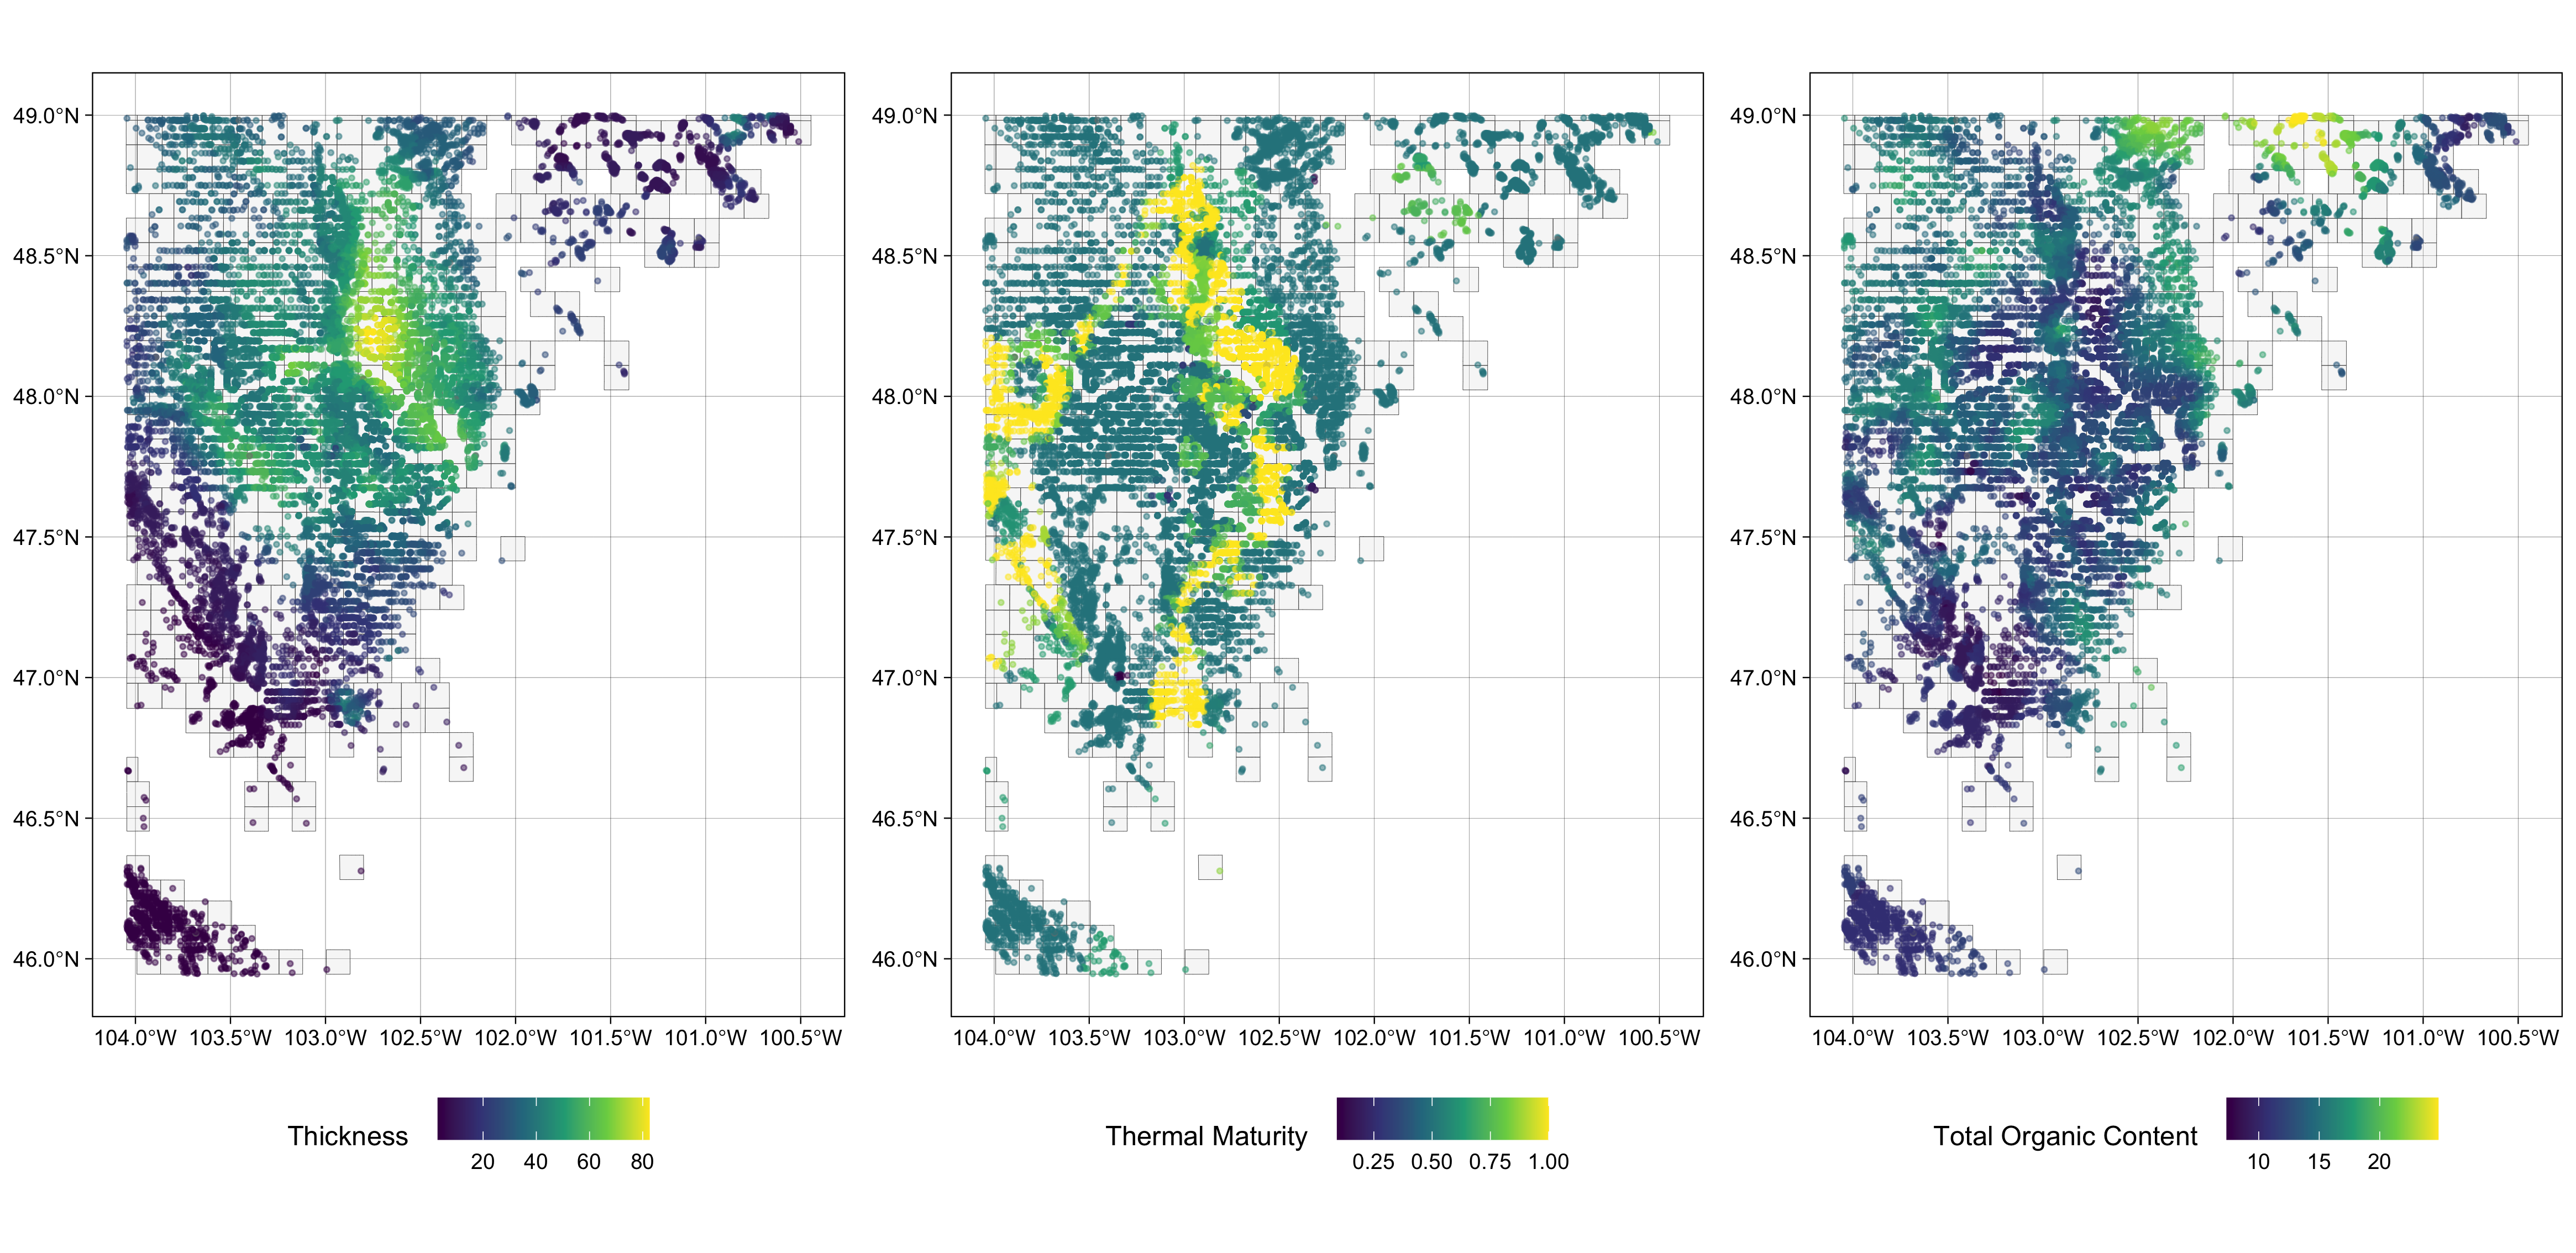
\includegraphics[scale = 0.13]{04_Chapter-3/00A_Figures/Figure_Spatial-Distributions-of-Geological-Characteristics.png}
        \caption{Spatial Distributions of Geological Characteristics}
        \caption*{
        	{\small
            \textit{Note}: 
            This figure depicts the spatial distributions of three geological features---thickness, thermal maturity, and total organic contents, which are available from the NDGS' geological survey data--- for the horizontal wells in our sample. In this figure, each square is a section in the Public Land Survey System, whereas each dot indicates an individual well's geological characteristic.  
        }}
        \label{Figure:Spatial-Distributions-of-Geological-Characteristics}
    \end{figure}
% }
\end{landscape}
